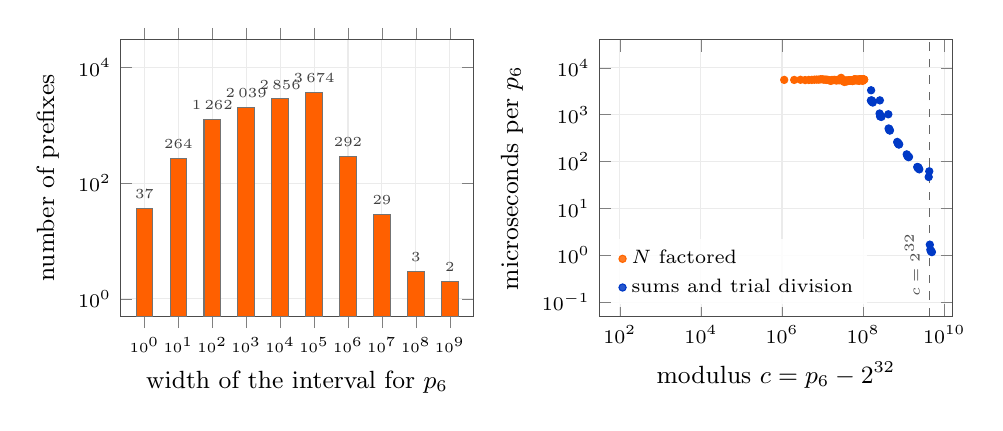
\begin{tikzpicture}
\begin{axis}[name=left, width=0.50\textwidth, height=0.42\textwidth, ybar, bar width=6pt, ymode=log, log origin=infty,
  ymin=0.5, ymax=3e4, xmin=-0.7, xmax=9.7,
  xtick={0,...,9}, xticklabels={$10^0$,$10^1$,$10^2$,$10^3$,$10^4$,$10^5$,$10^6$,$10^7$,$10^8$,$10^9$},
  x tick label style={font=\tiny}, y tick label style={font=\scriptsize}, axis line style={black!70},
  ylabel={\small number of prefixes}, xlabel={\small width of the interval for $p_6$},
  grid=major, grid style={black!8},
  nodes near coords={\pgfmathprintnumber[fixed, precision=0, 1000 sep={\,}]{\pgfplotspointmeta}},
  nodes near coords style={font=\tiny, text=black!75, anchor=south}, point meta=rawy]
\addplot[fill=orange!75!red, draw=black!55] coordinates {(0,37) (1,264) (2,1262) (3,2039) (4,2856) (5,3674) (6,292) (7,29) (8,3) (9,2)};
\end{axis}
\begin{axis}[at={(left.east)}, anchor=west, xshift=16mm, width=0.50\textwidth, height=0.42\textwidth,
  xmin=1.5, xmax=10.2, ymin=-1.3, ymax=4.6, axis line style={black!70},
  xtick={2,4,6,8,10}, xticklabels={$10^2$,$10^4$,$10^6$,$10^8$,$10^{10}$},
  ytick={-1,0,1,2,3,4}, yticklabels={$10^{-1}$,$10^0$,$10^1$,$10^2$,$10^3$,$10^4$},
  x tick label style={font=\scriptsize}, y tick label style={font=\scriptsize},
  xlabel={\small modulus $c=p_6-2^{32}$}, ylabel={\small microseconds per $p_6$},
  grid=major, grid style={black!8},
  legend style={font=\scriptsize, draw=none, fill=white, fill opacity=0.85, text opacity=1, at={(0.03,0.03)}, anchor=south west}, legend cell align=left]
\addplot[only marks, mark=*, mark size=1.3pt, color=orange!80!red] coordinates {(6.0535,3.7434) (6.2999,3.7426) (6.4552,3.7460) (6.5695,3.7395) (6.6607,3.7423) (6.7359,3.7436) (6.8000,3.7478) (6.8562,3.7504) (6.9066,3.7482) (6.9517,3.7577) (6.9925,3.7564) (7.0299,3.7491) (7.0642,3.7494) (7.0961,3.7451) (7.1257,3.7453) (7.1538,3.7363) (7.1804,3.7329) (7.2055,3.7231) (7.2292,3.7404) (7.2517,3.7385) (7.2731,3.7400) (7.2935,3.7443) (7.3129,3.7380) (7.3316,3.7357) (7.3494,3.7322) (7.3666,3.7438) (7.3831,3.7416) (7.3990,3.7385) (7.4143,3.7377) (7.4291,3.7403) (7.4434,3.7406) (7.4575,3.7869) (7.4712,3.7417) (7.4845,3.7290) (7.4974,3.7357) (7.5099,3.7229) (7.5221,3.7306) (7.5340,3.7000) (7.5455,3.7192) (7.5567,3.7311) (7.5677,3.7096) (7.5784,3.7279) (7.5888,3.7282) (7.5990,3.7111) (7.6089,3.7237) (7.6187,3.7247) (7.6282,3.7224) (7.6375,3.7237) (7.6466,3.7362) (7.6555,3.7331) (7.6643,3.7262) (7.6728,3.7291) (7.6813,3.7317) (7.6895,3.7348) (7.6976,3.7294) (7.7055,3.7275) (7.7133,3.7325) (7.7210,3.7318) (7.7285,3.7231) (7.7360,3.7184) (7.7432,3.7236) (7.7504,3.7387) (7.7574,3.7348) (7.7644,3.7460) (7.7714,3.7473) (7.7783,3.7502) (7.7850,3.7340) (7.7917,3.7555) (7.7982,3.7440) (7.8047,3.7512) (7.8110,3.7388) (7.8173,3.7478) (7.8235,3.7346) (7.8296,3.7495) (7.8356,3.7386) (7.8415,3.7404) (7.8473,3.7472) (7.8531,3.7369) (7.8588,3.7457) (7.8644,3.7474) (7.8700,3.7328) (7.8754,3.7410) (7.8808,3.7380) (7.8862,3.7410) (7.8915,3.7450) (7.8967,3.7511) (7.9018,3.7232) (7.9069,3.7451) (7.9120,3.7439) (7.9169,3.7534) (7.9218,3.7465) (7.9267,3.7437) (7.9315,3.7581) (7.9363,3.7433) (7.9410,3.7445) (7.9456,3.7524) (7.9502,3.7447) (7.9548,3.7364) (7.9593,3.7426) (7.9638,3.7400) (7.9682,3.7464) (7.9726,3.7546) (7.9769,3.7466) (7.9812,3.7437) (7.9854,3.7446) (7.9896,3.7228) (7.9938,3.7431) (7.9979,3.7388) (8.0020,3.7526) (8.0060,3.7504) (8.0100,3.7494) (8.0140,3.7487) (8.0180,3.7536) (8.0219,3.7517) (8.0257,3.7478)};
\addplot[only marks, mark=*, mark size=1.3pt, color=blue!55!teal] coordinates {(8.1913,3.3041) (8.1966,3.5218) (8.2019,3.2950) (8.2071,3.2988) (8.2123,3.3045) (8.2174,3.2763) (8.2224,3.2792) (8.2274,3.2749) (8.2323,3.2750) (8.2371,3.2602) (8.4059,3.0258) (8.4125,3.3066) (8.4191,2.9634) (8.4256,2.9760) (8.4319,2.9693) (8.4382,2.9716) (8.4444,2.9710) (8.4504,2.9539) (8.6208,3.0092) (8.6289,2.7070) (8.6369,2.6818) (8.6447,2.6952) (8.6523,2.6713) (8.6599,2.6615) (8.8407,2.4196) (8.8507,2.3995) (8.8604,2.3819) (8.8699,2.3914) (8.8792,2.3635) (8.8883,2.3702) (9.0743,2.1541) (9.0861,2.1362) (9.0977,2.1107) (9.1089,2.1077) (9.1199,2.0948) (9.1306,2.1007) (9.3338,1.8851) (9.3471,1.8639) (9.3600,1.8793) (9.3726,1.8474) (9.3847,1.8347) (9.6165,1.6716) (9.6305,1.7923) (9.6442,0.2274) (9.6575,0.1195) (9.6705,0.0853) (9.6830,0.0856) (9.6952,0.0684)};
\draw[black!60, dashed] (axis cs:9.633,-1.3) -- (axis cs:9.633,4.6);
\node[font=\tiny, text=black!70, anchor=south, rotate=90] at (axis cs:9.633,-0.2) {$c=2^{32}$};
\legend{$N$ factored, sums and trial division}
\end{axis}
\end{tikzpicture}
